\documentclass[times,onecolumn]{article}

\usepackage{graphicx}
\usepackage{amssymb}
\usepackage{lineno}

% Additional packages
\usepackage[american]{babel}
\usepackage[utf8]{inputenc}
\usepackage{amsmath}
\usepackage{currfile}
\usepackage{url}
\usepackage{rotfloat}
\usepackage{xcolor}
\usepackage{framed}
\usepackage{listings}
\usepackage{comment}
\usepackage{verbatim}
\usepackage{mdframed}
\usepackage{calc}

\usepackage{Sweave}
%\SweaveSyntax{SweaveSyntaxLatex}

\usepackage{caption}
\DeclareCaptionType[fileext=loc]{listing}

\definecolor{shadecolor}{gray}{0.9}

%\VignetteIndexEntry{A code generator for ODE-based models in R}

\begin{document}

% Turn prompts off in R code

\lstset{basicstyle=\ttfamily\small,
  commentstyle=\textsl,
  showstringspaces=false,
  frame=shadowbox,
  rulesepcolor=\color{black},
  rangebeginprefix= \#\#TexBegin\{,
  rangebeginsuffix= \},
  rangeendprefix= \#\#TexEnd\{,
  rangeendsuffix= \},
  includerangemarker= false,
  numbers=left,
  numberstyle=\color{white}\ttfamily\tiny,
  stepnumber=1,
  numbersep=3mm,
  morecomment=[is]{\#\#----------------------------------------BeginHide}
    {\#\#----------------------------------------EndHide}
}

\newcommand{\software}[1]{\texttt{#1}}

\newcommand{\figdir}{.}
\newcommand{\sect}{Section}
\newcommand{\sects}{Sections}

\newcommand{\oxygen}{O\ensuremath{_{2}}}
\newcommand{\OM}{\textrm{OM}}
\newcommand{\DO}{\textrm{DO}}

\newcommand{\todo}[1]{\textcolor{red}{\textbf{#1}}}

\newcommand{\grey}[1]{\textcolor{gray}{#1}}

\title{Vignette for \software{R} package \software{rodeo}}

\author{David Kneis, david.kneis [at] tu-dresden.de}

\date{\today}

\maketitle

\tableofcontents

\section{When to use this package}

The \software{rodeo} package facilitates the implementation of ODE-based models. These are models that describe the dynamics of a set of $n$ state variables by integrating a set of $n$  ordinary differential equations. The package is particularly useful in conjunction with the \software{deSolve} package (\url{http://cran.r-project.org/web/packages/deSolve/index.html}) providing numerical solvers for initial value problems. The advantages from using \software{rodeo} are:

\begin{itemize}
\item Models are defined using plain tabular text files or spreadsheets. Thus, the model is formulated independent from source code. This facilitates documentation, portability, and re-use.
\item You are forced to provide the model in stoichiometry matrix notation (see \url{http://en.wikipedia.org/wiki/Petersen_matrix}). Although this is a restriction, it is a very useful one and benefit is almost guaranteed.
\item Owing to the matrix notation, redundant terms are eliminated from the differential equations. This contributes to comprehensibility and increases computational efficiency. The stoichiometry matrix can also be visualized to better communicate the model to users or non-modelers.
\item \software{rodeo} provides a code generator which supports \software{R} and \software{Fortran} as target languages. Using compiled \software{Fortran} can speed up numerical integration by 1 or 2 orders of magnitude (compared to plain \software{R}).
\item The generated source code is applicable to an arbitrary number of boxes (control volumes). This allows even partial differential equations (e.~g. reactive transport problems) to be tackled by means of semi-discretization  (see \url{http://en.wikipedia.org/wiki/Method_of_lines}).
\end{itemize}

\section{Example problem}
The functioning of the package is best illustrated by an example. In this document, we consider a continuous flow stirred tank reactor (CFSTR) containing a degradable organic matter (concentration \verb|c_z|) and dissolved oxygen, \verb|c_do| (Fig.~\ref{fig:reactor}). Due to mixing, the reactors contents is spatially homogeneous, hence the concentrations are scalars. Changes in concentrations are triggered by
\begin{enumerate}
\item the loads in the reactor's inflow,
\item aerobic degradation of the organic matter (1st order) which consumes dissolved oxygen,
\item exchange of oxygen with the atmosphere.
\end{enumerate}

Some specific aspects of the model are as follows:
\begin{itemize}
\item The dependence of aerobic degradation on available oxygen is described with a Monod term (Michaelis-Menten model).
\item The rate of oxygen exchange between water and atmosphere is described as an empirical function of water depth and wind speed.
\item The model does \emph{not} assume steady flow conditions, hence the volume of the reactor is a state variable too.
\end{itemize}

\begin{figure}
\centering
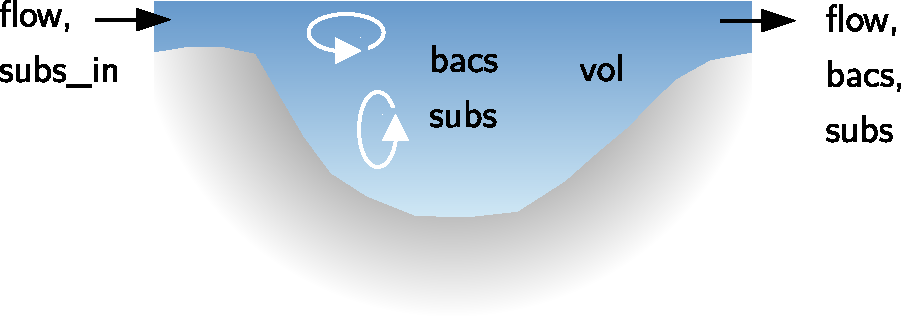
\includegraphics[width=0.5\textwidth]{reactor.pdf}
\caption{Sketch of considered system. \label{fig:reactor}}
\end{figure}

Using \software{rodeo}, the model can be described using just tabular text files (Tables~\ref{tab:identifiers} -- \ref{tab:stoichiometry}). These files are shipped with the package and can be loaded with \software{R}'s \verb|data| method.

\begin{table}
\caption{Declaration of identifiers (data set 'exampleIdentifiers'). The type column indicates whether an item is a state variable (v), parameter (p), or function (f). \label{tab:identifiers}}
\begin{shaded}
\begin{small}
\begin{Schunk}
\begin{Soutput}
    name type unit              description       tex              html
    c_do    v mg/l             dissolved O2    c_{DO}    c<sub>DO</sub>
     c_z    v mg/l degradable org. matter Z       c_Z     c<sub>Z</sub>
       v    v   m3  water volume in reactor         v                 v
    q_in    p m3/s              inflow rate    q_{in}    q<sub>in</sub>
    q_ex    p m3/s             outflow rate    q_{ex}    q<sub>ex</sub>
      kd    p  1/d               decay rate       k_d     k<sub>d</sub>
  s_do_z    p  g/g     stoichiometry (O2/Z)  s_{DO,Z}  s<sub>DO,Z</sub>
    h_do    p g/m3       half-saturation O2    h_{DO}    h<sub>DO</sub>
    temp    p degC              temperature         T                 T
    wind    p  m/s               wind speed         W                 W
   depth    p    m              water depth         D                 D
   O2sat    f mg/l   O2 saturation, f(temp)  O2_{sat}  O2<sub>sat</sub>
      ka    f  1/d aeration, f(wind, depth)       k_a     k<sub>a</sub>
   monod    f    -              monod model     monod             monod
  c_z_in    f g/m3     Z in inflow, f(time)  c_{Z,in}  c<sub>Z,in</sub>
 c_do_in    f g/m3    O2 in inflow, f(time) c_{DO,in} c<sub>DO,in</sub>
\end{Soutput}
\end{Schunk}
\end{small}
\end{shaded}
\end{table}

\begin{table}
\caption{Specification of processes (data set 'exampleProcesses'). \label{tab:processes}}
\begin{shaded}
\begin{small}
\begin{Schunk}
\begin{Soutput}
     name   unit   description                            expression
     flow   m3/s water balance                           q_in - q_ex
 flushing    1/s flushing rate                              q_in / v
    decay g/m3/s    decay of z          kd * c_z * monod(c_do, h_do)
 aeration g/m3/s   O2-exchange ka(wind,depth) * (O2sat(temp) - c_do)
\end{Soutput}
\end{Schunk}
\end{small}
\end{shaded}
\end{table}

\begin{table}
\caption{Specification of stoichiometric factors (data set 'exampleStoichiometry'). \label{tab:stoichiometry}}
\begin{shaded}
\begin{small}
\begin{Schunk}
\begin{Soutput}
 variable  process           expression
        v     flow                    1
      c_z flushing   c_z_in(time) - c_z
      c_z    decay                   -1
     c_do flushing c_do_in(time) - c_do
     c_do    decay              -s_do_z
     c_do aeration                    1
\end{Soutput}
\end{Schunk}
\end{small}
\end{shaded}
\end{table}


%%%%%%%%%%%%%%%%%%%%%%%%%%%%%%%%%%%%%%%%%%%%%%%%%%%%%%%%%%%%%%%%%%%%%%%%%
%%%%%%%%%%%%%%%%%%%%%%%%%%%%%%%%%%%%%%%%%%%%%%%%%%%%%%%%%%%%%%%%%%%%%%%%%
%%%%%%%%%%%%%%%%%%%%%%%%%%%%%%%%%%%%%%%%%%%%%%%%%%%%%%%%%%%%%%%%%%%%%%%%%

\clearpage
\section{Basic use}

\subsection{Creating and inspecting a model object}

We start by creating a new object with \verb|new|. This requires us to supply the name of the class as well as a set of data frames for initialization.

\begin{Schunk}
\begin{Sinput}
 library(rodeo, quietly=TRUE)
 # Load sample data frames (contents shown above)
 data(exampleIdentifiers, exampleProcesses, exampleStoichiometry)
 # Instantiate new object
 model= new("rodeo", vars=subset(exampleIdentifiers,type=="v"),
   pars=subset(exampleIdentifiers,type=="p"),
   funs=subset(exampleIdentifiers,type=="f"),
   pros=exampleProcesses, stoi=exampleStoichiometry)
\end{Sinput}
\end{Schunk}

To inspect the object's contents, we can use the following:

\begin{Schunk}
\begin{Sinput}
 # Built-in method
 model$show()
 # Show stoichiometry information as a matrix
 print(model$stoichiometry())
\end{Sinput}
\end{Schunk}

\subsection{Defining functions and supplying data}

In order to work with the object, we need to define functions that are referenced in the model's mathematical expressions. This includes the forcings which are functions of a special argument with the reserved name 'time'. See Sect.~\ref{sec:advanced:forcings} for details.

\begin{Schunk}
\begin{Sinput}
 # 'normal' functions
 O2sat= function(t) {
   14.652 - 0.41022*t + 0.007991*t^2 - 0.000077774*t^3
 }
 ka= function(u, d) {
   (0.728*sqrt(u) - 0.317*u + 0.0372*u^2) / d / 86400
 }
 monod= function(s,h) {
   s / (s + h)
 }
\end{Sinput}
\end{Schunk}

\begin{Schunk}
\begin{Sinput}
 # forcings are functions of special variable 'time'
 c_z_in= function(seconds) {
   0.1 * seconds/(7*86400 + seconds)
 }
 c_do_in= function(seconds) {
   10.  # taken as constant
 }
\end{Sinput}
\end{Schunk}

We also need to set the values of parameters and state variables (initial values). We first define both parameters and initial values as lists. These lists are then coerced into named vectors using the dedicated methods \verb|arrangePars| and \verb|arrangeVars|. Use of these methods guarantees that the vector elements appear in proper order. Proper order is essential when the vector elements are accessed \emph{by position} rather than \emph{by name}.

\begin{Schunk}
\begin{Sinput}
 pars= list(kd=5.78e-7, h_do=0.5, s_do_z=2.76, wind=1, depth=2,
  temp=20, q_in=1, q_ex=1)
 vars= list(c_z=1, c_do=9.022, v=1.e6)
 p= model$arrangePars(pars)
 v= model$arrangeVars(vars)
\end{Sinput}
\end{Schunk}

\subsection{Computing the stoichiometry matrix}

Having defined all functions and having set the values of variables and parameters, one can compute the stoichiometric factors. In general, explicitly computing these factors is not necessary, it may be helpful in debugging however. To do so, the \verb|stoichiometry| method needs to be supplied with values of all state variables, parameters, as well as a time value (in the case of non-autonomous models).

\begin{Schunk}
\begin{Sinput}
 m= model$stoichiometry(c(v, p, time=0))
 print(signif(m, 3))
\end{Sinput}
\begin{Soutput}
           c_do c_z v
flow      0.000   0 1
flushing  0.978  -1 0
decay    -2.760  -1 0
aeration  1.000   0 0
\end{Soutput}
\end{Schunk}

The stoichiometry matrix is also a good means to communicate a model because it shows the interactions between processes and variables in a concise way. How the stoichiometry matrix can be visualized graphically is demonstrated in Sect.~\ref{sec:advanced:doc:stoi}.

\subsection{Translating the model into source code}

In order to use the model for simulation, we need to transfer it into source code. This is also known as \emph{code generation}. Specifically, we want the code generator to create a function that returns the derivatives of the state variables with respect to time. In addition to the derivatives, the generated function also returns the values of all process rates (as diagnostic variables).

After generating the code, we need to make it executable. In \software{R}, we can use a combination of \verb|eval| and \verb|parse|. Alternatively, the generated code could be for loaded with \verb|source| after exporting it to a file (e.g. using \verb|write|). The latter method is needed if one wants to inspect the generated code (or even modify it, which rarely makes sense).

\begin{Schunk}
\begin{Sinput}
 code= model$generate(name="derivs",lang="r")
 derivs= eval(parse(text=code))
\end{Sinput}
\end{Schunk}

\subsection{Solving the ODE system} \label{sec:solve-R}

We are now ready to compute the evolution of the state variables over time by means of numerical integration. At this point, the proper order of the elements in the vectors \verb|v| and \verb|p| is essential since the generated function code uses \emph{by-index} access! Therefore, \verb|v| and \verb|p| should always be set by calls to the \verb|arrangeVars| and \verb|arrangePars| method, respectively.

In addition to the dynamics of the state variables, we also get the dynamics of the process rates.

\begin{Schunk}
\begin{Sinput}
 library(deSolve)
 t= seq(0, 30*86400, 3600)
 out= ode(y=v, times=t, func=derivs, parms=p, NLVL=1)
 layout(matrix(1:9, ncol=3, byrow=TRUE))
 plot(out, mfrow=NULL)
 layout(1)
\end{Sinput}
\end{Schunk}
\includegraphics{rodeo-012}

%%%%%%%%%%%%%%%%%%%%%%%%%%%%%%%%%%%%%%%%%%%%%%%%%%%%%%%%%%%%%%%%%%%%%%%%%
%%%%%%%%%%%%%%%%%%%%%%%%%%%%%%%%%%%%%%%%%%%%%%%%%%%%%%%%%%%%%%%%%%%%%%%%%
%%%%%%%%%%%%%%%%%%%%%%%%%%%%%%%%%%%%%%%%%%%%%%%%%%%%%%%%%%%%%%%%%%%%%%%%%

\clearpage
\section{Advanced topics} \label{sec:advanced}

%%%%%%%%%%%%%%%%%%%%%%%%%%%%%%%%%%%%%%%%%%%%%%%%%%%%%%%%%%%%%%%%%%%%%%%%%
%%%%%%%%%%%%%%%%%%%%%%%%%%%%%%%%%%%%%%%%%%%%%%%%%%%%%%%%%%%%%%%%%%%%%%%%%

\subsection{Spatially distributed systems (multi-box models)} \label{sec:advanced:multibox}

A zero-dimensional case (single reactor) has been considered so far. We will now extend the model for multiple spatial levels, i.~e. for a collection of (isolated) reactors.

First, we need to provide vectors (instead of scalars) for one variable and one parameter, at least. Variables and parameters with scalar values will be replicated to vectors of the required length. In the example, we initialize every modeled reactor with a different concentration of organic matter.

Second, we need to pass the actual number of reactors to the derivatives function in the \verb!NLVL! argument.

\begin{Schunk}
\begin{Sinput}
 nbox= 3
 pars= list(kd=rep(5.78e-7, nbox), h_do=0.5, s_do_z=2.76, wind=1,
   depth=2, temp=20, q_in=1, q_ex=1)
 vars= list(c_z=seq(from=0, to=50, length.out=nbox), c_do=9.022,
   v=1.e6)
 p= model$arrangePars(pars)
 v= model$arrangeVars(vars)
 out= ode(y=v, times=t, func=derivs, parms=p, NLVL=nbox)
 layout(matrix(1:nbox, nrow=1))
 plot(out, which=paste("c_do",1:nbox,sep="."), mfrow=NULL)
\end{Sinput}
\end{Schunk}
\includegraphics{rodeo-014}

%%%%%%%%%%%%%%%%%%%%%%%%%%%%%%%%%%%%%%%%%%%%%%%%%%%%%%%%%%%%%%%%%%%%%%%%%
%%%%%%%%%%%%%%%%%%%%%%%%%%%%%%%%%%%%%%%%%%%%%%%%%%%%%%%%%%%%%%%%%%%%%%%%%

\subsection{Increasing performance by means of Fortran} \label{sec:advanced:fortran}

Real-world models usually consist of many and lengthy mathematical expressions. Also, depending on the studied problem, the ODE solver may need to use (very) short time steps. Then, computation times become of serious concern. In those time-critical cases, it is recommended to generate source code for a fast, compilable language rather than for (slower) \software{R}. The compilable language supported by \software{rodeo} is \software{Fortran}.

The next statement generates \software{Fortran} code and exports it to a file for later compilation.

\begin{Schunk}
\begin{Sinput}
 code= model$generate(name="derivs",lang="f95")
 file_fdrvs= "derivatives.f95"
 write(x=code, file=file_fdrvs)
 # Optionally display generated code
 #cat(code)
\end{Sinput}
\end{Schunk}

Inspection of the generated \software{Fortran} code reveals that the interface of the central subroutine \verb|derivs| is

\begin{verbatim}
subroutine derivs(time, var, par, NLVL, dydt, pro)
\end{verbatim}

However, according to the \software{deSolve} vignette \url{http://cran.r-project.org/web/packages/deSolve/vignettes/compiledCode.pdf}, page 6, the following interface is required

\begin{verbatim}
subroutine derivs (neq, t, y, ydot, yout, ip)
\end{verbatim}

and an additional subroutine for parameter initialization (\verb|initmod|) must to be supplied as well. Consequently, we need to provide the following \software{Fortran} code:

\begin{enumerate}
\item a wrapper around the generated derivatives function to make its interface compatible with \software{deSolve},
\item the additional subroutine \verb|initmod| for parameter initialization,
\item any functions being referenced in the particular model's mathematical expressions (consult Sect.~\ref{sec:fortranFunctions} for guidelines).
\end{enumerate}

A suitable Fortan code for (1) and (2) can be generated by the function call \verb|solverInterface(NLVL)| where the integer argument \verb|NLVL| specifies the desired number of spatial levels (see Sect.~\ref{sec:advanced:multibox}; default is \verb|NLVL=1|). The generated wrapper and initialization code must be written to disk for later use by the compiler.

\begin{Schunk}
\begin{Sinput}
 # Generate wrapper and initialization routine
 fwrap= solverInterface(nbox, "derivs")
 # Optionally display the generated code
 #cat(fwrap)
 # Export generated code to file for later compilation
 file_fwrap= "fwrap.f95"
 write(fwrap, file_fwrap)
\end{Sinput}
\end{Schunk}

The model-specific functions (number 3 in above list) could be defined as:

\begin{shaded}
\begin{Schunk}
\begin{Soutput}
module functions 
   implicit none 
   contains 
  
   double precision function O2sat(t)  
     double precision, intent(in):: t 
     O2sat= 14.652d0 - 0.41022d0*t + 7.991d-3*(t**2d0) - & 
       7.7774d-5*(t**3d0) 
   end function 
  
   double precision function ka(u, d)  
     double precision, intent(in):: u, d 
     ka= (0.728d0*sqrt(u) - 0.317d0*u + 0.0372d0*(u**2.d0)) / & 
       d / 86400.d0 
   end function 
  
   double precision function monod(s, h)  
     double precision, intent(in):: s, h 
     monod= s / (s + h) 
   end function 
  
   double precision function c_z_in(seconds)  
     double precision, intent(in):: seconds 
     c_z_in= 0.1d0 * seconds/(7d0*86400d0 + seconds) 
   end function 
  
   double precision function c_do_in(seconds)  
     double precision, intent(in):: seconds 
     c_do_in= 10.d0 
   end function 
  
 end module 
\end{Soutput}
\end{Schunk}
\end{shaded}

Note that all functions are collected in a single \software{Fortran} module with implicit typing turned off. The name of this module (\verb|functions|) is mandatory and cannot be changed.

As a next step, one needs to compile the generated code and the hand-coded functions into a shared library. For that purpose, we make use of \software{R}'s command line utility \verb|R CMD SHLIB|. The 3 files passed to the command are the following:

\medskip
\begin{tabular}{lp{0.7\textwidth}}
\verb|file_fdrvs| & File containing the derivatives function (automatically created with the \verb|generate| class method, see above) \\
\verb|file_fwrap| & Source file containing the wrapper and initialization routine (automatically created with the \verb|solverIterface| method, see above) \\
\verb|file_ffuns| & Hand-coded source file with the model-specific function (contents shown above) \\
\end{tabular}

\begin{Schunk}
\begin{Sinput}
 dllname= "mySharedLib"
 dllfile= paste0(dllname,.Platform$dynlib.ext)
 command= paste0("R CMD SHLIB ",file_ffuns," ",file_fdrvs," ",
   file_fwrap," --preclean --clean -o ",dllfile)
 if (system(command) != 0)
   stop(paste0("Error running '",command,"'"))
\end{Sinput}
\end{Schunk}


We are now prepared to load the shared library and run the simulation based on the Fortran code. Note the additional arguments \verb|dllname|, \verb|initfunc|, and \verb|nout| being passed to the numerical solver (open the help page for \verb|lsoda| to see the documentation for them). Setting a wrong value for \verb|nout| easily makes \software{R} crash.

Also note that, in contrast to the R-based version (see Sect.~\ref{sec:solve-R}), the number of reactors (boxes) is not passed to the solver as an additional parameter \verb|NLVL|. In the case of Fortran, this number is rather supplied to the \verb|solverInterface| method (see above) and it is thus hard-coded in the compiled code.

\begin{Schunk}
\begin{Sinput}
 nbox= 3
 pars= list(kd=rep(5.78e-7, nbox), h_do=0.5, s_do_z=2.76, wind=1,
   depth=2, temp=20, q_in=1, q_ex=1)
 vars= list(c_z=seq(from=0, to=50, length.out=nbox), c_do=9.022,
   v=1.e6)
 p= model$arrangePars(pars)
 v= model$arrangeVars(vars)
 dyn.load(dllfile)
 out= ode(y=v, times=t, func="derivs_wrapped", parms=p,
   dllname=dllname, initfunc="initmod", nout=model$lenPros()*nbox)
 layout(matrix(1:nbox, nrow=1))
 dyn.unload(dllfile)
 plot(out, which=paste("c_do",1:nbox,sep="."), mfrow=NULL)
\end{Sinput}
\end{Schunk}
\includegraphics{rodeo-020}


%%%%%%%%%%%%%%%%%%%%%%%%%%%%%%%%%%%%%%%%%%%%%%%%%%%%%%%%%%%%%%%%%%%%%%%%%
%%%%%%%%%%%%%%%%%%%%%%%%%%%%%%%%%%%%%%%%%%%%%%%%%%%%%%%%%%%%%%%%%%%%%%%%%

\subsection{Forcings (time-varying parameters)} \label{sec:advanced:forcings}

\subsubsection{Two alternative options}
In general, there are two options for dealing with time-variable forcings:

\paragraph{functions-of-time:} In this approach one needs to define the forcings as functions of a single argument representing time. In \software{rodeo} this argument must have the reserved name \verb|time|. Use of this approach is most convenient if the forcings are easily described as parametric functions of time (e.g. seasonal change of solar radiation). It can also be used with tabulated time series data, but this requires some extra coding. In any case, it is essential for rescrict the integration step size of the solver (e.g. using the \verb|hmax| argument of \verb|deSolve::lsoda|) so that short-term variations in the forcings cannot be 'missed'.
 
\paragraph{stop-and-go:} In this approach forcings are implemented as normal parameters. To allow for their variation in time, the ODE solver is interrupted every time when the forcing data change. The solver is then re-started with the updated parameters (i.e. forcing data) using the states computed in the previous call as initial values. Hence, the calls to the ODE solver must be embedded within a time-loop. With this approach, setting a limit on the solver's integration step size (through argument \verb|hmax|) is not required since the solver is interrupted at the 'critical times' anyway.

In real-world applications, the 'stop-and-go' approach is often simpler to use and the overhead due to interruption and re-start of the solvers seems to be rather small. It also facilitates the generation of useful traceback information in case of exceptions (e.g. due to corrupt time series data).

\subsubsection{The 'functions-of-time' approach with Fortran models}

This section demonstrates how the 'functions-of-time' approach can be used in Fortran-based models assuming that information on forcings is stored in delimited text files. Such files can be created, for example, with any spreadsheet software, data base system, or \software{R}. Assume that we have time series of two meteorological variables exported to a text file 'meteo.txt':

\begin{Schunk}
\begin{Sinput}
 dat= data.frame(time=1:10, temp=round(rnorm(n=10, mean=20, sd=3)),
   humid=round(runif(10)*100))
 write.table(x=dat, file="meteo.txt", col.names=TRUE,
   row.names=FALSE, sep="\t", quote=FALSE)
 print(dat)
\end{Sinput}
\begin{Soutput}
   time temp humid
1     1   24    31
2     2   21     3
3     3   18    39
4     4   23     7
5     5   21    49
6     6   20    39
7     7   21    11
8     8   19    73
9     9   13    78
10   10   20     3
\end{Soutput}
\end{Schunk}

We can now call \verb|forcingFunctions| to generate the  appropriate forcing function in \software{Fortran}. In this example, we request linear interpolation via the method's \verb|mode| argument.

\begin{Schunk}
\begin{Sinput}
 dat= data.frame(name=c("temp","humid"),
   column=c("temp","humid"), file="meteo.txt", mode=-1, default=FALSE)
 code= forcingFunctions(dat)
 write(x=code, file="forc.f95")
 # Optionally inspect generated code
 # cat(code)
\end{Sinput}
\end{Schunk}

In order to use the generated code, it is necessary to
\begin{enumerate}
\item write it to disk (e.~g. using \verb|write| as above),
\item declare all forcings as functions in \software{rodeo}'s respective input table,
\item insert the statement \verb|use forcings| at the top (e.~g. line 2) of the \software{Fortran} module \verb|functions|,
\item pass the generated file to the compiler along with all other \software{Fortran} source files.
\end{enumerate}

The following Fortran code demonstrates how the user-defined forcings can be tested/debugged outside of the \software{rodeo} environment. The shown utility program can be compiled, for example, using a command like

\medskip
\verb|gfortran <generated_module_file> <file_with_program> -o test|

\medskip
Note that the subroutines \verb|rwarn| and \verb|rexit| are available automatically if the code is used to build a shared library with \verb|R CMD SHLIB|, i.~e. the subroutines must not be defined then.

\begin{shaded}
\begin{Schunk}
\begin{Soutput}
 ! auxiliary routines for testing outside R 
 subroutine rwarn(x) 
   character(len=*),intent(in):: x 
   write(*,*)x 
 end subroutine 
  
 subroutine rexit(x) 
   character(len=*),intent(in):: x 
   write(*,*)x 
   stop 
 end subroutine 
  
 ! test program 
 program test 
 use forcings  ! imports generated module with forcing functions 
  
 implicit none 
  
 integer:: i 
 double precision, dimension(5):: times= & 
   dble((/ 1., 1.5, 2., 2.5, 3. /)) 
  
 do i=1, size(times) 
   write(*,*) times(i), temp(times(i)), humid(times(i)) 
 end do 
 end program 
\end{Soutput}
\end{Schunk}
\end{shaded}

%%%%%%%%%%%%%%%%%%%%%%%%%%%%%%%%%%%%%%%%%%%%%%%%%%%%%%%%%%%%%%%%%%%%%%%%%
%%%%%%%%%%%%%%%%%%%%%%%%%%%%%%%%%%%%%%%%%%%%%%%%%%%%%%%%%%%%%%%%%%%%%%%%%

\subsection{Generating model documentation} \label{sec:advanced:doc}

\subsubsection{Exporting formatted tables} \label{sec:advanced:doc:tables}

One can use e.g. \verb|exportDF| to export the object's basic information in a format which is suitable for inclusion in HTML or \LaTeX{} documents. The code section

\begin{Schunk}
\begin{Sinput}
 # Select columns to export
 df= model$getVars()[,c("tex","unit","description")]
 # Define formatting functions
 bold= function(x){paste0("\\textbf{",x,"}")}
 mathmode= function(x) {paste0("$",x,"$")}
 # Export
 tex= exportDF(x=df, tex=TRUE,
   colnames=c(tex="symbol"),
   funHead=setNames(replicate(ncol(df),bold),names(df)),
   funCell=list(tex=mathmode)
 )
 cat(tex)
\end{Sinput}
\end{Schunk}

generates the following \LaTeX{} code holding tabular information on the model's state variables.

\begin{shaded}
\begin{Schunk}
\begin{Soutput}
  \begin{tabular}{lll}\hline
    \textbf{symbol} & \textbf{unit} & \textbf{description} \\ \hline
    $c_{DO}$ & mg/l & dissolved O2 \\
    $c_Z$ & mg/l & degradable org. matter Z \\
    $v$ & m3 & water volume in reactor \\ \hline
  \end{tabular}
\end{Soutput}
\end{Schunk}
\end{shaded}

Alternatively, a \software{markdown} compatible dataframe can be generated and used with the \software{knitr} function \verb|kable|. This will work with html, pdf or even Word (.docx) output. The code section

\begin{Schunk}
\begin{Sinput}
 to_markdown= function(dat, which_cols){
   cols= which(names(dat) %in% which_cols)
   for(i in cols){
     dat[, i]= ifelse(dat[, i] != "", paste0("$", dat[, i], "$"), "")
     }
   return(dat)
 } 
 ids= model$getVars()[,c("tex", "unit", "description")]
 names(ids)= c("Symbol", "Unit", "Description")
 kable(to_markdown(ids, which_cols=c("Symbol")),
   caption = "State variables")
\end{Sinput}
\end{Schunk}

generates the following \software{markdown} code:

\begin{shaded}
\begin{Schunk}
\begin{Soutput}
|Symbol   |Unit |Description              |
|:--------|:----|:------------------------|
|$c_{DO}$ |mg/l |dissolved O2             |
|$c_Z$    |mg/l |degradable org. matter Z |
|$v$      |m3   |water volume in reactor  |
\end{Soutput}
\end{Schunk}
\end{shaded}

Thanks to Andrew Dolman for the latter example.

\subsubsection{Visualizing the stoichiometry matrix} \label{sec:advanced:doc:stoi}

A graphical representation of the stoichiometry matrix is often a good means to communicate a model. To create such a graphics, one typically wants to replace the stoichiometry factors' numeric values by symbols encoding their sign only.

\paragraph{Option 1: Plain R graphics}
One can use the class method \verb|plotStoichiometry| to visualize the matrix using standard R graphic facilities as demonstrated below. In practice, one needs to fiddle around a bit with the dimensions of the plot and the font size to get an acceptable scaling of symbols and text. Also, it is hardly possible to nicely display row and column names containing special things like sub- or superscripts.

\begin{Schunk}
\begin{Sinput}
 pars= list(kd=5.78e-7, h_do=0.5, s_do_z=2.76, wind=1, depth=2,
  temp=20, q_in=1, q_ex=1)
 vars= list(c_z=1, c_do=9.022, v=1.e6)
 p= model$arrangePars(pars)
 v= model$arrangeVars(vars)
 model$plotStoichiometry(values=c(v, p, time=0), cex=0.3)
\end{Sinput}
\end{Schunk}
\includegraphics{rodeo-029}

\paragraph{Option 2: TEX}
The following example generates suitable code for inclusion in \LaTeX{} documents.

\begin{Schunk}
\begin{Sinput}
 pars= list(kd=5.78e-7, h_do=0.5, s_do_z=2.76, wind=1, depth=2,
  temp=20, q_in=1, q_ex=1)
 vars= list(c_z=1, c_do=9.022, v=1.e6)
 p= model$arrangePars(pars)
 v= model$arrangeVars(vars)
 signsymbol= function(x) {
   if (as.numeric(x) > 0) return("\\textcolor{orange}{$\\blacktriangle$}")
   if (as.numeric(x) < 0) return("\\textcolor{cyan}{$\\blacktriangledown$}")
   return("")
 }
 rot90= function(x) { paste0("\\rotatebox{90}
   {$",gsub(pattern="*", replacement="\\cdot ", x=x, fixed=TRUE),"$}") }
 m= model$stoichiometry(c(v, p, time=0))
 tbl= cbind(data.frame(process=rownames(m), stringsAsFactors=FALSE),
   as.data.frame(m))
 tex= exportDF(x=tbl, tex=TRUE,
   colnames= setNames(c("",model$getVars()$tex[match(colnames(m),
     model$getVars()$name)]), names(tbl)),
   funHead= setNames(replicate(ncol(m),rot90), colnames(m)),
   funCell= setNames(replicate(ncol(m),signsymbol), colnames(m)),
   lines=TRUE
 )
 tex= paste0("%\n% THIS IS A GENERATED FILE\n%\n", tex)
 # write(tex, file="/home/dkneis/temp/stoichiometry.tex")
\end{Sinput}
\end{Schunk}

The contents of the variable \verb|tex| must be written to a text file and this file is then imported in \LaTeX{} with the \verb|input| directive. The result looks as follows:

\begin{center}
%
% THIS IS A GENERATED FILE
%
  \begin{tabular}{lrrr}\hline
     & \rotatebox{90}
  {$c_{DO}$} & \rotatebox{90}
  {$c_Z$} & \rotatebox{90}
  {$v$} \\ \hline
    flow &  &  & \textcolor{orange}{$\blacktriangle$} \\
    flushing & \textcolor{orange}{$\blacktriangle$} & \textcolor{cyan}{$\blacktriangledown$} &  \\
    decay & \textcolor{cyan}{$\blacktriangledown$} & \textcolor{cyan}{$\blacktriangledown$} &  \\
    aeration & \textcolor{orange}{$\blacktriangle$} &  &  \\ \hline
  \end{tabular}


\end{center}

\paragraph{Option 3: HTML}

The following example generates suitable code for inclusion in HTML documents.

\begin{Schunk}
\begin{Sinput}
 signsymbol= function(x) {
   if (as.numeric(x) > 0) return("&#9651;")
   if (as.numeric(x) < 0) return("&#9661;")
   return("")
 }
 m= model$stoichiometry(c(v, p, time=0))
 tbl= cbind(data.frame(process=rownames(m), stringsAsFactors=FALSE),
   as.data.frame(m))
 html= exportDF(x=tbl, tex=FALSE,
   colnames= setNames(c("Process",model$getVars()$html[match(colnames(m),
     model$getVars()$name)]), names(tbl)),
   funCell= setNames(replicate(ncol(m),signsymbol), colnames(m))
 )
 html= paste("<html>", html, "</html>", sep="\n")
 # write(html, file="/home/dkneis/temp/stoichiometry.html")
\end{Sinput}
\end{Schunk}

To test this, one needs to write the contents of the variable \verb|html| to a text file and open that file in a web browser. In some cases, automatic conversion of the generated HTML into true graphics formats may be possible, e.~g. using auxiliary tools like \software{html2ps} and \software{convert} (on Linux systems).

\paragraph{Option 4: Markdown}

A \software{markdown} compatible version looks like this (contributed by Andrew Dolman):

\begin{Schunk}
\begin{Sinput}
 signsymbol= function(x) {
   if (as.numeric(x) > 0) return("$\\blacktriangle$")
   if (as.numeric(x) < 0) return("$\\blacktriangledown$")
   return("")
 }
 stoi_mat= model$stoichiometry(c(v, p, time=0))
 stoi_mat= data.frame(apply(stoi_mat, MARGIN = c(1, 2), signsymbol))
 stoi_mat= setNames(stoi_mat, paste0("$",     
   model$getVars()$tex[match(colnames(stoi_mat),
   model$getVars()$name)], "$"))
 stoi_mat= cbind(Process=rownames(stoi_mat), stoi_mat)
 kable(stoi_mat, row.names= FALSE, caption= "Stoichiometric matrix")
\end{Sinput}
\end{Schunk}

and the generated \software{markdown} output is:

\begin{shaded}
\begin{small}
\begin{Schunk}
\begin{Soutput}
|Process  |$c_{DO}$             |$c_Z$                |$v$              |
|:--------|:--------------------|:--------------------|:----------------|
|flow     |                     |                     |$\blacktriangle$ |
|flushing |$\blacktriangle$     |$\blacktriangledown$ |                 |
|decay    |$\blacktriangledown$ |$\blacktriangledown$ |                 |
|aeration |$\blacktriangle$     |                     |                 |
\end{Soutput}
\end{Schunk}
\end{small}
\end{shaded}

%%%%%%%%%%%%%%%%%%%%%%%%%%%%%%%%%%%%%%%%%%%%%%%%%%%%%%%%%%%%%%%%%%%%%%%%%
%%%%%%%%%%%%%%%%%%%%%%%%%%%%%%%%%%%%%%%%%%%%%%%%%%%%%%%%%%%%%%%%%%%%%%%%%
%%%%%%%%%%%%%%%%%%%%%%%%%%%%%%%%%%%%%%%%%%%%%%%%%%%%%%%%%%%%%%%%%%%%%%%%%

\section{Writing \software{rodeo}-compatible \software{Fortran} functions} \label{sec:fortranFunctions}

\subsection{Reference example}

As a reference, the following example code can be used which declares a function of two arguments. Comments have been added to explain the individual statements. In Fortran, comments are generally initiated with the exclamation mark (!). They may appear right after statements or on separate lines.

\begin{shaded}
\begin{small}
\begin{verbatim}
1  double precision function FUNCNAME (ARG1, ARG2) ! declare the function
2  implicit none                                   ! force declarations
3  double precision, intent(in):: ARG1, ARG2       ! declare arguments
4  double precision:: LOCAL                        ! declare local var.
5  double precision, parameter:: CONST=1.d0        ! declare local const.
6  LOCAL= ARG1 * CONST + ARG2                      ! local computation(s)
7  FUNCNAME= LOCAL                                 ! set return value
8  end function                                    ! closes the function
\end{verbatim}
\end{small}
\end{shaded}

For compatibility with \software{rodeo}, the function result must be a scalar of type \verb|double precision| (a floating point number of typically 8 byte). There are several ways to achieve this but the simplest and recommended syntax is put the type declaration \verb|double precision| right before the function's name (line 1). Then, the return value must be set by an assignment to the function's name (line 7). This is best done at a single location in the body code, typically at the very end.

It is a good habit to always put \verb|implicit none| in the first line of the function body (line 2). This is to disable so-called implicit typing (a rather dangerous technique of automatic data type assignment). With this statement, all arguments (line 3) and local variables or constants (lines 4 and 5) need to be explicitly declared. The repetition of the argument's names in lines 1 and 3 may be a bit annoying (but one can use copy and paste). All declarations need to be made at the top of the function's body (right after the \verb|implicit none|) before any other statements.

In \software{Fortran}, identifier names are not case-sensitive (as opposed to \software{R}). This applies to the name of the function itself as well as to the names of arguments and local variables or parameters.

Note: It is actually sufficient to use the \verb|implicit none| statement at the beginning of the module that contains all function declarations (see example in Sect.~\ref{sec:advanced:fortran}). Repetition of the statement in the individual functions does not do any harm, however. 

\subsection{Common pitfalls}

\subsubsection{Double precision variables and constants}

Fortran has several types to represent floating point numbers that vary in precision but \software{rodeo} generally uses the type \verb|double precision|. Thus, any local variables and parameters should also be declared as \verb|double precision|. To declare a numeric constant of this type, e.~g. 'pi', one needs to use the syntax \verb|3.1415d0|, i.~e. the conventional 'e' in scientific notation is replaced by 'd'. An alternative but less portable syntax exists but it is not mentioned here.

\begin{shaded}
\begin{small}
\begin{verbatim}
double precision, parameter:: pi= 3.1415d0, e= 2.7183d0   ! math constants 
double precision, parameter:: kilograms_per_gram = 1.d-3  ! 1/1000
double precision, parameter:: distance_to_moon = 3.844d+5 ! 384400 km
\end{verbatim}
\end{small}
\end{shaded}

Note the \verb|parameter| keyword used to inform the compiler that the declared item(s) are constants rather than variables.

\subsubsection{Integers in numeric expressions}

It is recommended to avoid integers in arithmetic expressions as the result may be unexpected. Use \verb|double precision| constants instead of \verb|integer| constants or, alternatively, explicitly convert \verb|integer| constants to \verb|double precision| by means of the \verb|dble| intrinsic function.

\begin{shaded}
\begin{small}
\begin{verbatim}
average= (value1 + value2) / 2d0       ! does not use an integer at all
average= (value1 + value2) / dble(2)   ! explicit type conversion
\end{verbatim}
\end{small}
\end{shaded}

It is often even better not to use any literal constants, leading to a code like

\begin{shaded}
\begin{small}
\begin{verbatim}
double precision, parameter:: TWO= 2.d0
! possibly other statements
average= (value1 + value2) / TWO
\end{verbatim}
\end{small}
\end{shaded}

Using uppercase names for constants is a widespread habit but this is a matter of style only.

\subsubsection{Continuation lines}

Source code lines should not exceed 80 characters (though some \software{Fortran} compilers support longer lines). If an expression does not fit on a single line, the ampersand (\verb|&|) must be used to indicate continuation lines. It is recommended to put the \verb|&| at the end of any unfinished line as in the following example:

\begin{shaded}
\begin{small}
\begin{verbatim}
a = term1 + term2 + &
    term3 + term4 + &
    term5
\end{verbatim}
\end{small}
\end{shaded}

Missing \verb|&| characters are a frequent cause of compile time errors sometimes being rather obscure.

\subsection{More information on \software{Fortran} programming}

The examples in Sect.~\ref{sec:advanced:fortran} may serve as a starting point. The website \url{http://fortranwiki.org/fortran/show/HomePage} is a good source of additional information, providing links to standard documents, books, etc.

%%%%%%%%%%%%%%%%%%%%%%%%%%%%%%%%%%%%%%%%%%%%%%%%%%%%%%%%%%%%%%%%%%%%%%%%%
%%%%%%%%%%%%%%%%%%%%%%%%%%%%%%%%%%%%%%%%%%%%%%%%%%%%%%%%%%%%%%%%%%%%%%%%%
%%%%%%%%%%%%%%%%%%%%%%%%%%%%%%%%%%%%%%%%%%%%%%%%%%%%%%%%%%%%%%%%%%%%%%%%%

\section{Practical issues} \label{sec:practical}

\subsection{Managing tabular input data}

The tabular input data can be held in either plain text files or spreadsheets. The two alternatives have their own pros and cons as described below:

Spreadsheet software is specialized on displaying tabular data in a convenient way. Nevertheless, there are some practical issues. For example, spreadsheet programs allow for cell formatting. Formatting rules and automatisms often lead to unwanted results (e.g. in the case of logical columns). This also depends on the used format (e.g. 'xlsx' or 'odt'). As of now, R does not have native support for spreadsheets in 'odt' format. Conversion between 'odt' and 'xlsx' is possible, but the exact result seems to be unpredictable.

Delimited text files are much simpler in concept. They can be edited with any editor and platform dependence is a minor issue because line endings and character encodings are easy to change. Good programs provide powerful editing commands, e.g. using regular expressions, and they can highlight matching parenthesis. Text files are perfect for use with version control systems. Nevertheless, normal editors are unable to display tabular data in a nice way.

It is a good compromise to store the tabular data in delimited text files (e.g. separated by TAB or semicolon) and to open them either in a spreadsheet program or editor, depending on the actual task. Note that the conventional 'csv' is not recommended since mathematical expressions involving multi-argument functions and text descriptions may contain commas (hence, they need to be quoted). Using TAB-delimited text is probably the best option.

\end{document}

